\documentclass[8pt]{beamer}
\usepackage{url}
\usepackage{graphicx}
\usepackage{mhchem}
\usepackage{multicol}

\usetheme{Madrid}
\usefonttheme{serif}

% Configuração da fonte
\usepackage{fontspec}
%\setmainfont{Times New Roman} % Fonte Times New Roman
\setmainfont{Arial} % Fonte Arial (descomente esta linha se preferir Arial)

% Configuração do espaçamento de linhas
\usepackage{setspace}
\onehalfspacing % Espaçamento 1,5 entre linhas
%\singlespacing % Espaçamento simples (1 entre linhas)
%\doublespacing % Espaçamento duplo (2 entre linhas)

\begin{document}

\title[Chembl Database]{\LARGE Relatório de Caracterização de DataBase usando R}
\author[Lucas Galvão Janot]{Lucas Galvão Janot}
\institute[CEUB]{CEUB}
\date{\today}

\begin{frame}
  \titlepage
\end{frame}

\begin{frame}{Introduction}
  \begin{itemize}
    \item Database escolhida: Chembl.
    \item Contém informações sobre moléculas bioativas e suas propriedades.
    \item Database pode ser encontrada em \url{https://www.ebi.ac.uk/chembl/}.
    \item Gerenciado pelo Laboratório Europeu de Biologia Molecular - Instituto Europeu de Bioinformática (EMBL-EBI).
    \item Mais de 2 milhões de registros distintos.
    \item Amplamente utilizado no desenvolvimento de medicamentos e pesquisas em química medicinal.
  \end{itemize}
\end{frame}

\begin{frame}{Database Information}
  \begin{itemize}
    \item Nome da Database: ChEMBL
    \item Data de lançamento: Oct 2009
    \item Data da última versaõ: Jan 2023
    \item Responsável: Instituto Europeu de Bioinformática do Laboratório Europeu de Biologia Molecular (EMBL-EBI).
    \item Objetivo: Fornecer um recurso abrangente e de acesso livre de moléculas bioativas com propriedades semelhantes a medicamentos e suas atividades biológicas associadas para descoberta e desenvolvimento de medicamentos.
  \end{itemize}
\end{frame}

\begin{frame}{Variables used for the analysis}
  \begin{itemize}
    \item \textbf{ChEMBL ID}: Identificador único para cada entrada de composto
    \item \textbf{Name}: Nome da molécula
    \item \textbf{SMILES}: Sistema de Entrada de Linha de Fórmula Molecular Simplificada
    \item \textbf{Molecular Formula}: Representação da composição da molécula
    \item \textbf{Molecular Weight}: Massa da molécula
    \item \textbf{ALogP}: Coeficiente de Partição Aquosa
    \item \textbf{NumHAcceptors}: Número de sítios aceitadores de ligação de hidrogênio
    \item \textbf{NumHDonors}: Número de sítios doadores de ligação de hidrogênio
    \item \textbf{NumRotatableBonds}: Número de ligações que podem girar livremente
    \item \textbf{RingCount}: Número de anéis presentes na molécula
    \item \textbf{TPSA}: Área de Superfície Polar Topológica
    \item \textbf{Type}: Classificação da molécula com base em sua estrutura química e características.
  \end{itemize}
\end{frame}

\begin{frame}{Árvore de Variáveis}
  \begin{center}
    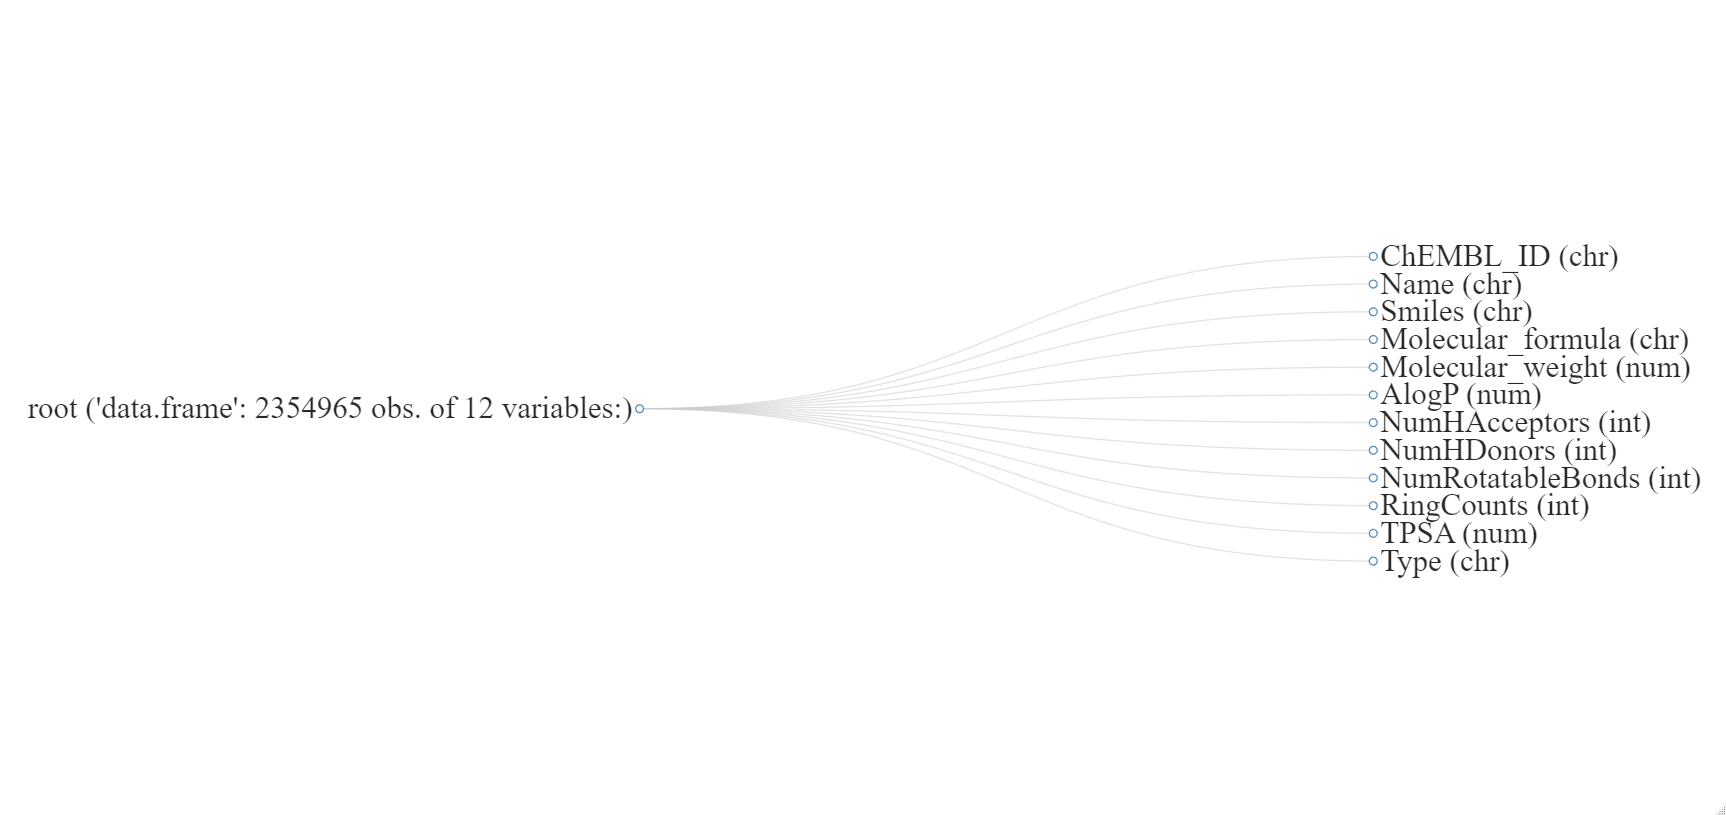
\includegraphics[width=1\textwidth, ]{variables.png}
  \end{center}
\end{frame}

\begin{frame}{Resumo das Variáveis}
\begin{multicols}{2}
  \begin{itemize}
    \item \textbf{ChEMBL ID}:
      \begin{itemize}
        \item Length: 2,354,965
        \item Class: Character
        \item Mode: Character
        \item NA's: 0
      \end{itemize}
    \item \textbf{Name}:
      \begin{itemize}
        \item Length: 2,354,965
        \item Class: Character
        \item Mode: Character
        \item NA's: 0
      \end{itemize}
      \item \textbf{SMILES:}
    \begin{itemize}
        \item \textbf{Length:} 2,354,965
        \item \textbf{Class:} Character
        \item \textbf{Mode:} Character
        \item \textbf{NA`s:} 0
    \end{itemize}
     \item \textbf{Molecular Formula:}
    \begin{itemize}
        \item \textbf{Length:} 2,354,965
        \item \textbf{Class:} Character
        \item \textbf{Mode:} Character
        \item \textbf{NA`s:} 0
    \end{itemize}
  \end{itemize}
  \end{multicols}
\end{frame}

\begin{frame}{Resumo das Variáveis (cont.}
\begin{multicols}{2}
  \begin{itemize}
     \item \textbf{Molecular Weight:}
    \begin{itemize}
        \item \textbf{Min.:} 4.0 (CHEMBL1796997, Name: Undefined, \ce{He} , Small Molecule)
        \item \textbf{1st Qu.:} 324.4
        \item \textbf{Median:} 392.4
        \item \textbf{Mean:} 433.9
        \item \textbf{3st Qu.:} 474.5
        \item \textbf{Max.:} 12546.3 (CHEMBL2179464, Name: Undefined, \ce{C396H390F252N66O24P42}, Small Molecule)
        \item \textbf{NA`s:} 23,442 ($\approx 1\% $)
    \end{itemize}
     \item \textbf{ALogP:}
    \begin{itemize}
        \item \textbf{Min.:} -14.26 (CHEMBL1797815, Name: CELLOHEXOSE, \ce{C36H62O31} , Small Molecule)
        \item \textbf{1st Qu.:} 2.31
        \item \textbf{Median:} 3.42
        \item \textbf{Mean:} 3.45
        \item \textbf{3st Qu.:} 4.57
        \item \textbf{Max.:} 22.57 (CHEMBL1206998, Name: Undefined  \ce{C64H127NO3S}, Small Molecule)
        \item \textbf{NA`s:} 84,994 ($\approx 3.61\% $)
    
    \end{itemize}
  \end{itemize}
  \end{multicols}
\end{frame}

\begin{frame}{Resumo das Variáveis (cont.)}
\begin{multicols}{2}
  \begin{itemize}
         \item \textbf{NumHAcceptors:}
    \begin{itemize}
        \item \textbf{Min.:} 0.0 (CHEMBL425822, Name: Undefined, \ce{C36H62O31} , Small Molecule)
        \item \textbf{1st Qu.:} 4.0
        \item \textbf{Median:} 5.0
        \item \textbf{Mean:} 5.5
        \item \textbf{3st Qu.:} 6.0
        \item \textbf{Max.:} 32 (CHEMBL604420, Name: Undefined, \ce{C24H16F6}, Small Molecule)
        \item \textbf{NA`s:} 84,994 ($\approx 3.61\% $)
    \end{itemize}
    \columnbreak
    \item \textbf{NumHDonors:}
    \begin{itemize}
        \item \textbf{Min.:} 0.0 (CHEMBL149936, Name: Undefined, \ce{C21H18N2O4S2} , Small Molecule)
        \item \textbf{1st Qu.:} 1.0
        \item \textbf{Median:} 1.0
        \item \textbf{Mean:} 1.59
        \item \textbf{3st Qu.:} 2.0
        \item \textbf{Max.:} 25 (CHEMBL1162334, Name: GUANIDINONEOMYCIN, \ce{C29H58N18O13}, Small Molecule)
        \item \textbf{NA`s:} 84,994 ($\approx 3.61\% $)
    \end{itemize}
  \end{itemize}
  \end{multicols}
\end{frame}


\begin{frame}{Resumo das Variáveis (contd.)}
\begin{multicols}{2}
  \begin{itemize}
  \item \textbf{NumRotatableBonds:}
    \begin{itemize}
        \item \textbf{Min.:} 0.0 (CHEMBL373674, Name: Undefined, \ce{C12H10N2O} , Small Molecule)
        \item \textbf{1st Qu.:} 3.0
        \item \textbf{Median:} 5.0
        \item \textbf{Mean:} 5.73
        \item \textbf{3st Qu.:} 7.0
        \item \textbf{Max.:} 67 (CHEMBL541380, Name: Undefined, \ce{C56H129ClN14}, Small Molecule)
        \item \textbf{NA`s:} 84,994 ($\approx 3.61\% $)
    \end{itemize}
    \item \textbf{RingCount:}
    \begin{itemize}
        \item \textbf{Min.:} 0.0 (CHEMBL409633, Name: Undefined, \ce{C74H12O} , Small Molecule)
        \item \textbf{1st Qu.:} 2.0
        \item \textbf{Median:} 2.0
        \item \textbf{Mean:} 2.46
        \item \textbf{3st Qu.:} 3.0
        \item \textbf{Max.:} 30 (CHEMBL409633, Name: Undefined, \ce{C74H12O}, Small Molecule)
        \item \textbf{NA`s:} 84,994 ($\approx 3.61\% $)
    \end{itemize}
     \item \textbf{TPSA:}
    \begin{itemize}
        \item \textbf{Min.:} 0.0 (CHEMBL425822, Name: Undefined, \ce{C24H16F6} , Small Molecule)
        \item \textbf{1st Qu.:} 54.88
        \item \textbf{Median:} 75.21
        \item \textbf{Mean:} 81.87
        \item \textbf{3st Qu.:} 99.27
        \item \textbf{Max.:} 595.22 (CHEMBL32709, Name: Undefined, \ce{C36H74N24O7}, Protein)
        \item \textbf{NA`s:} 84,994 ($\approx 3.61\% $)
    \end{itemize}
  \end{itemize}
  \end{multicols}
\end{frame}

\begin{frame}{Resumo das Variáveis (contd.)}
  \begin{itemize}
    \item \textbf{Type:}
    \begin{itemize}
        \item \textbf{Length:} 2,354,965
        \item \textbf{Class:} Character
        \item \textbf{Mode:} Character
        \item \textbf{NA`s:} 0
        \item \textbf{Proportions:}
        \begin{multicols}{2}
            \begin{itemize}
                \item \textbf{Small Molecules:} 1,920,599 ($\approx 81.555\% $)
                \item \textbf{Unknown:} 409,991 ($\approx 17.41\% $)
                \item \textbf{Protein:} 22,750 ($\approx 0.966\% $)
                \item \textbf{Oligosaccharide:} 95 ($\approx 0.004\% $)
                \item \textbf{Oligonucleotide:} 201 ($\approx 0.009\% $)
                \item \textbf{Gene:} 107 ($\approx 0.005\% $)
                \item \textbf{Enzyme:} 121 ($\approx 0.005\% $)
                \item \textbf{Cell:} 55 ($\approx 0.002\% $)
                \item \textbf{Antibody:} 1046 ($\approx 0.044\% $)
            \end{itemize}
         \end{multicols}
     \end{itemize}
  \end{itemize}
\end{frame}


\begin{frame}{Histogramas}
\begin{figure}[h]
  \centering
  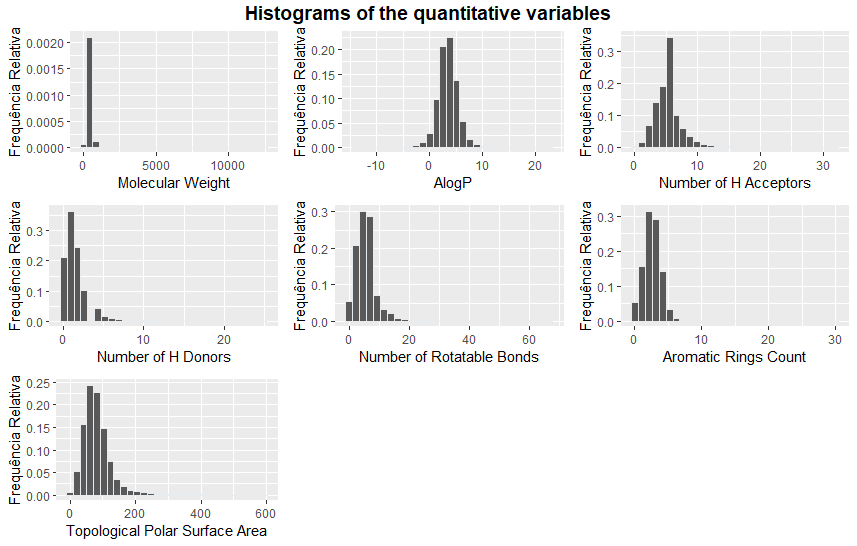
\includegraphics[width=\textwidth]{histogram.png}
\end{figure}
\end{frame}

\begin{frame}{Histogramas (cont.)}
\begin{figure}[h]
  \centering
  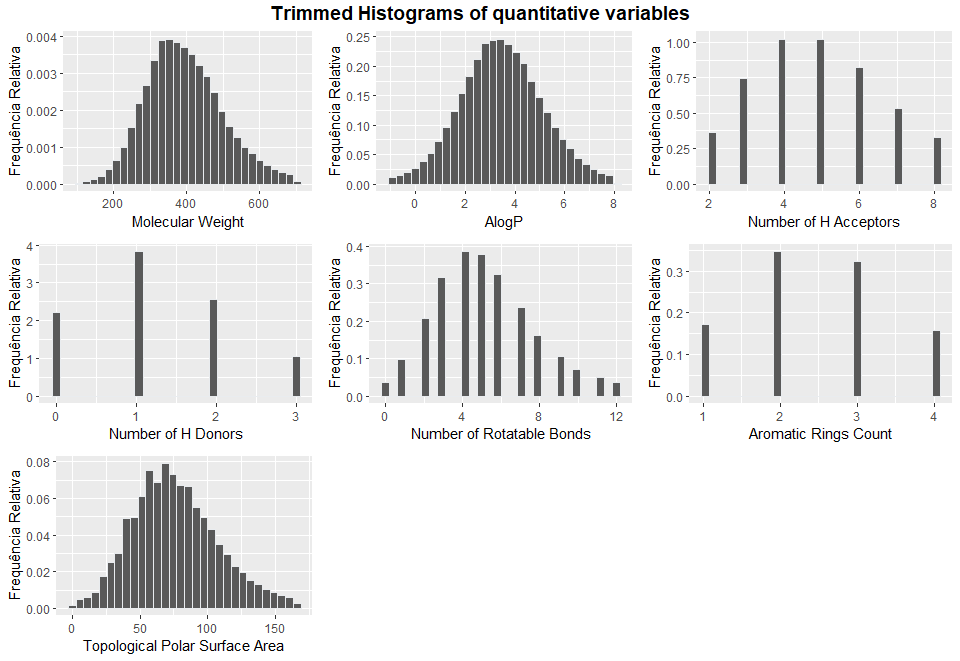
\includegraphics[width=\textwidth, height = 200pt]{trimmed.png}
\end{figure}
\end{frame}


\begin{frame}{Boxplot}
\begin{figure}[h]
  \centering
  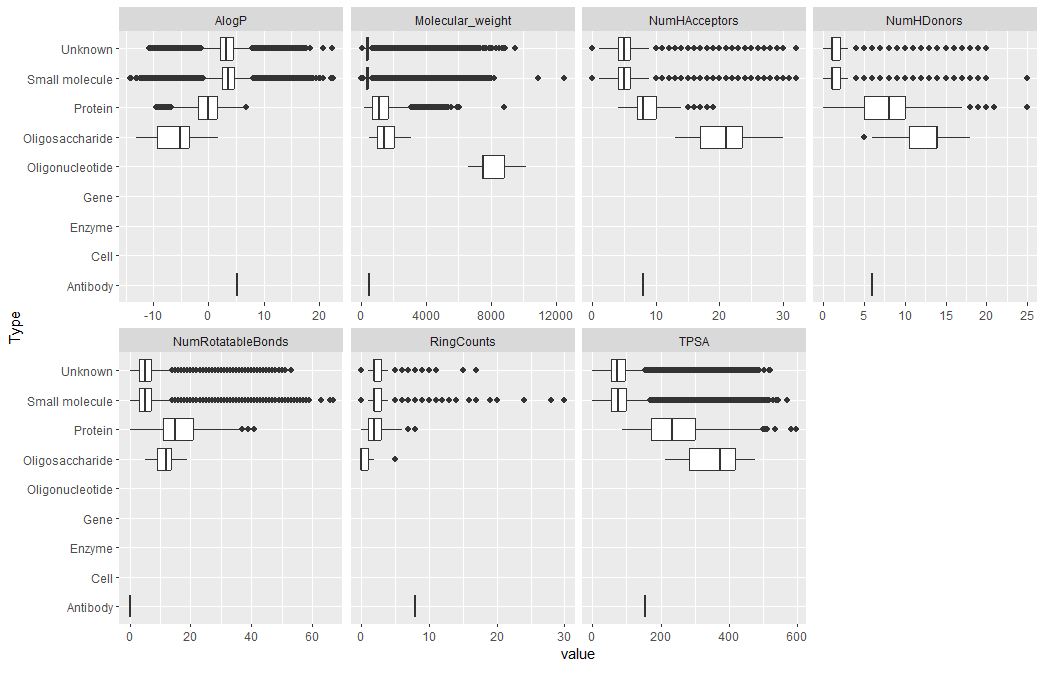
\includegraphics[width=\textwidth, height = 200pt]{boxplot.png}
\end{figure}
\end{frame}

\begin{frame}{Matrix de Correlação}
\begin{figure}[h]
  \centering
  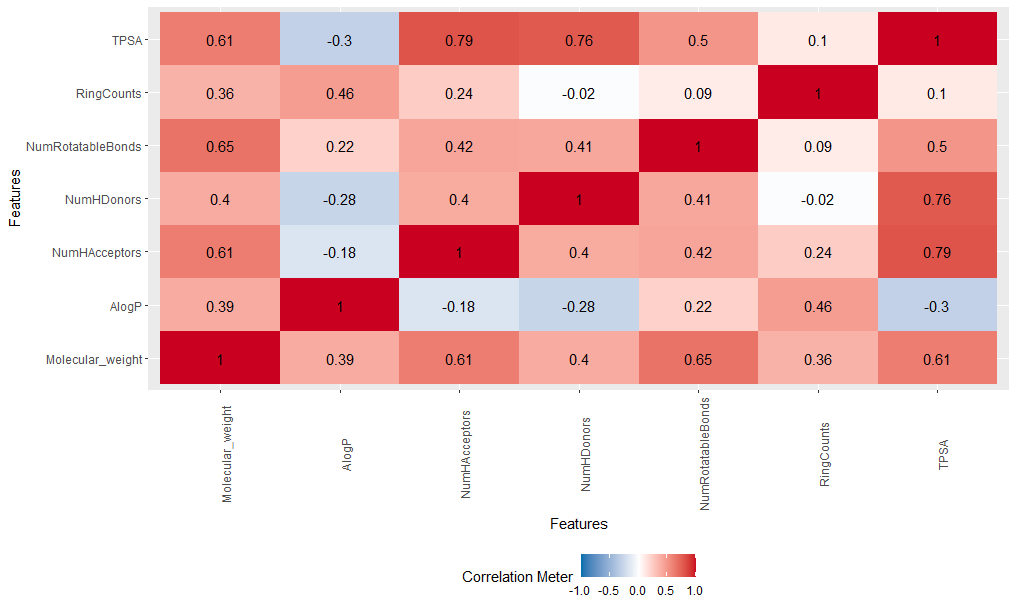
\includegraphics[width=\textwidth, height = 200pt]{correlation.png}
\end{figure}
\end{frame}

\begin{frame}{Scatter plots}
\begin{figure}[h]
  \centering
  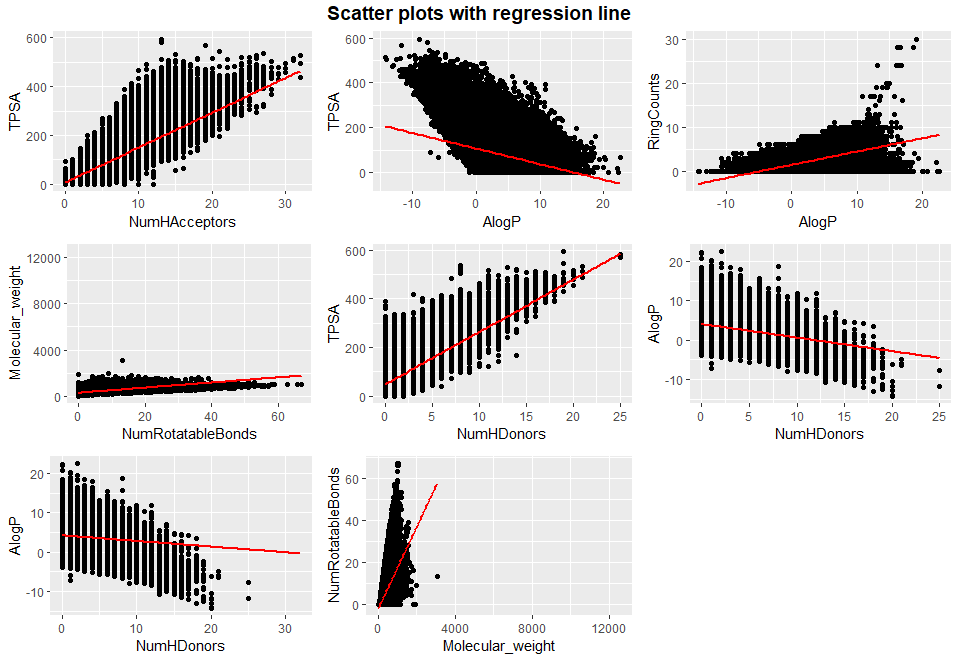
\includegraphics[width=\textwidth, height = 200pt]{regression.png}
\end{figure}
\end{frame}

\end{document}
